\documentclass{article}
\usepackage[utf8]{inputenc}
\usepackage{tikz}
\usetikzlibrary{shapes.geometric, arrows}

\tikzstyle{start_op} = [rectangle, minimum width=1cm, minimum height=1cm,text centered, draw=black]

\begin{document}
\begin{tikzpicture}[node distance=2cm]
% \draw (0,0) -- (0,4);
% \draw[thick] (0,0) -- (4,4);

% \draw[fill=red] (0,0) rectangle (3,4);

% \draw (0,0) parabola (4,4);

% \draw[<->] (0,0) -- (4,4);

\draw (0,0) .. controls (0,3) and (0,6)  .. (4,4);

\draw[black,ultra thick] (0,0) circle (5cm);

% \draw (2,2) ellipse (3cm and 1cm);

% \draw (3,0) circle (3cm);
% \draw (3,0) arc (0:75:3cm);

% \draw[step=1cm,gray,very thin] (-1.9,-1.9) grid (5.9,5.9);

% \filldraw[red] (2,2) circle (3cm);

% \shadedraw[inner color=blue,outer color=red, draw=black] (0,0) rectangle (4,4);

\draw[thick,->] (-8,0) -- (8,0) node[anchor=north west] {$x$ axis};
\draw[thick,->] (0,-8) -- (0,8) node[anchor=south east] {$y$ axis};
\draw[step=2.5cm, gray, thin] (-7.5,-7.5) grid (7.5,7.5);
\foreach \x in {-1, -1/2, 0, 1/2, 1}
    \draw (\x*5 cm,1pt) -- (\x*5 cm,-1pt) node[anchor=north] {$\x$};
\foreach \y in {-1, -1/2, 0, 1/2, 1}
    \draw (1pt,\y*5 cm) -- (-1pt,\y*5 cm) node[anchor=west] {$\y$};

\end{tikzpicture}
\\
% \lipsum[2]
\\


\\
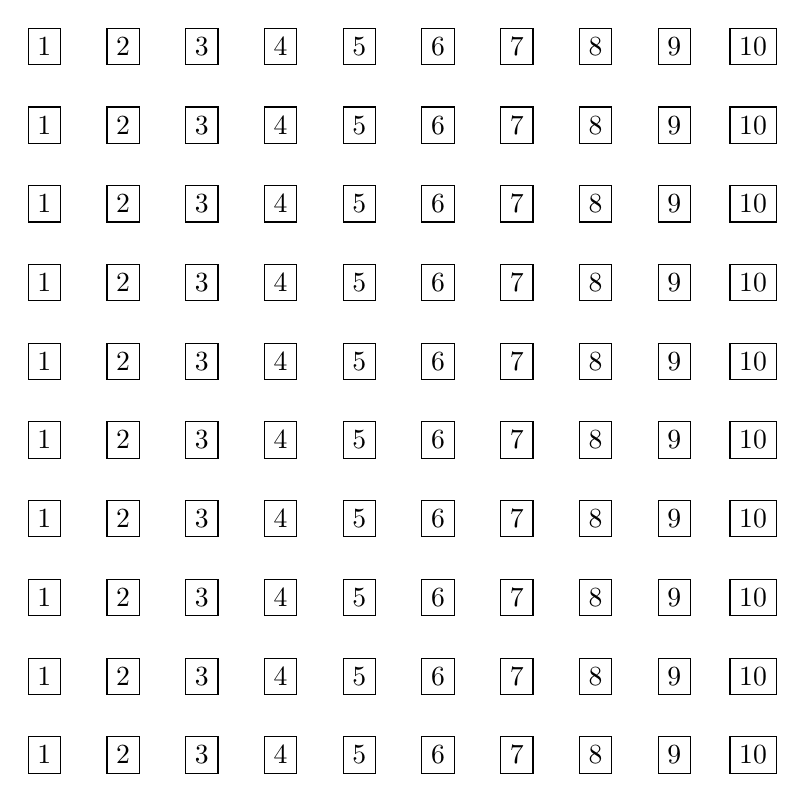
\begin{tikzpicture}
% \node (1) [start_op, right of = 0, xshift=1cm] {1};
% \node (2) [start_op, right of = 1, xshift=1cm] {2};
% \node (1) [start_op, right of = 0, xshift=1cm] {1};
% \node (1) [start_op, right of = 0, xshift=1cm] {1};
% \node (1) [start_op, right of = 0, xshift=1cm] {1};
% \node (1) [start_op, right of = 0, xshift=1cm] {1};
% \node (1) [start_op, right of = 0, xshift=1cm] {1};
 \foreach \j in {1,...,10}
 {
     \foreach \i in {1,...,10}
          {
             \node[draw,shape=rectangle] at (\i,\j) {\i};
          }
}
\end{tikzpicture}

\end{document}